\documentclass{article}
\usepackage{graphicx}
\usepackage{amsmath,amsthm,amssymb}
\usepackage[font=small,labelfont=bf]{caption}
\usepackage{tikz}
\usetikzlibrary{calc, angles, quotes, shapes.geometric, decorations.pathreplacing}
\usepackage{tkz-euclide}
\usepackage[inline]{asymptote}
\usepackage{float}
\usepackage[margin=1in]{geometry}
\usepackage{gensymb}
\usepackage[normalem]{ulem}
\usepackage{hyperref}
\hypersetup{
    colorlinks=true,
    linkcolor=blue,
    filecolor=magenta,      
    urlcolor=cyan,
    pdftitle={Overleaf Example},
    pdfpagemode=FullScreen,
    }
\usepackage{fancyhdr}
\pagestyle{fancy}
\fancyhead[R]{Enoch Yu}
\pagenumbering{gobble}
\usepackage{enumitem}
\newtheorem{theorem}{Theorem}[section]
\newtheorem{lemma}[theorem]{Lemma}
\newtheorem*{lemma*}{Lemma}
\newtheorem{sublemma}{Lemma}[section]
\newtheorem{proposition}{Proposition}
\newtheorem{corollary}{Corollary}[theorem]
\newtheorem{example}{Example}[section]
\newtheorem*{example*}{Example}
\newenvironment{solution}{\begin{trivlist}\item[]{\bf Solution}}{\qed \end{trivlist}}
\newcommand{\verteq}{\rotatebox{90}{$\;\;=\;\;$}}
\newcommand*\circled[1]{\tikz[baseline=(char.base)]{
            \node[shape=circle,draw,inner sep=1pt] (char) {#1};}}
\newcommand{\triangled}[1]{\tikz[baseline=(char.base)]{
            \node[shape=regular polygon, regular polygon sides=3, draw, inner sep=0.2pt] (char) {#1};}}

\title{Problem Set 20}
\author{Enoch Yu}
\date{June 2025}

\begin{document}

\section*{Basic Trigonometric Identities}
\begin{align*}
    \tan\theta &= \frac{\sin\theta}{\cos\theta} \\
    \sin^2\theta + \cos^2\theta &= 1 \\
    \frac{\sin^2\theta + \cos^2\theta}{\sin^2\theta} &\Rightarrow 1 + \cot^2\theta = \csc^2\theta \\
    \frac{\sin^2\theta + \cos^2\theta}{\cos^2\theta} &\Rightarrow \tan^2\theta + 1 = \sec^2\theta
\end{align*}
\[
\left\{
\begin{array}{l}
\sin(2\pi + \theta) = \sin\theta \\
\cos(2\pi + \theta) = \cos\theta \\
\tan(\pi + \theta) = \tan\theta
\end{array}
\right.
\qquad
\left\{
\begin{array}{l}
\sin(-\theta) = -\sin\theta \\
\cos(-\theta) = \cos\theta \\
\tan(-\theta) = -\tan\theta
\end{array}
\right.
\]

\[
\left\{
\begin{array}{l}
\sin(\pi - \theta) = \sin\theta \\
\cos(\pi - \theta) = -\cos\theta \\
\tan(\pi - \theta) = -\tan\theta
\end{array}
\right.
\qquad
\left\{
\begin{array}{l}
\sin\left(\frac{\pi}{2} - \theta\right) = \cos\theta \\
\cos\left(\frac{\pi}{2} - \theta\right) = \sin\theta \\
\tan\left(\frac{\pi}{2} - \theta\right) = \frac{1}{\tan\theta}
\end{array}
\right.
\]

\begin{example*}
    \[
    \text{Calculate }(1-\sin^2\theta)(1+\tan^2\theta).
    \]
\end{example*}
\begin{solution}
    \begin{align*}
        (1-\sin^2\theta)(1+\tan^2\theta)
        &= 1 + \tan^2\theta - \sin^2\theta - \sin^2\theta\tan^2\theta \\
        &= \sec^2\theta - \sin^2\theta(1 + \tan^2\theta) \\
        &= \sec^2\theta - \sin^2\theta\sec^2\theta \\
        &= \sec^2\theta(1 - \sin^2\theta) \\
        &= \sec^2\theta \cdot \cos^2\theta \\
        &= \boxed{1}
    \end{align*}
\end{solution}

\newpage
\begin{example*}
    \text{Prove that}
    \[
    \frac{1 + \tan\theta}{1 - \tan\theta} = \frac{1 + 2\sin\theta\cos\theta}{\cos^2\theta - \sin^2\theta}.
    \]
\end{example*}
\begin{proof}
    \begin{align*}
        \frac{1 + \tan\theta}{1 - \tan\theta}
        &= \frac{1 + \frac{\sin\theta}{\cos\theta}}{1 - \frac{\sin\theta}{\cos\theta}} \\
        &= \frac{\cos\theta + \sin\theta}{\cos\theta - \sin\theta} \\
        &= \frac{\cos\theta + \sin\theta}{\cos\theta - \sin\theta} \cdot \frac{\cos\theta + \sin\theta}{\cos\theta + \sin\theta} \\
        &= \frac{\cos^2\theta + 2\sin\theta\cos\theta + \sin^2\theta}{\cos^2\theta - \sin^2\theta} \\
        &= \boxed{\frac{1 + 2\sin\theta\cos\theta}{\cos^2\theta - \sin^2\theta}}
    \end{align*}
\end{proof}

\begin{example*}
    \text{Let $\sin\theta + \cos\theta = \frac{1}{2}$. Compute}
    \[
    \sin^6\theta + \cos^6\theta.
    \]
\end{example*}
\begin{solution}
    \begin{align*}
        (\sin\theta + \cos\theta)^2 &= \frac{1}{4} \\
        \sin^2\theta + 2\sin\theta\cos\theta + \cos^2\theta &= \frac{1}{4} \\
        2\sin\theta\cos\theta &= -\frac{3}{4} \\
        \sin\theta\cos\theta &= -\frac{3}{8}
        \\\\
        \sin^6\theta + \cos^6\theta
        &= (\sin^2\theta)^3 + (\cos^2\theta)^3 \\
        &= (\sin^2\theta + \cos^2\theta)^3 - 3\sin^2\theta\cos^2\theta(\sin^2\theta + \cos^2\theta) \\
        &= 1 - 3\sin^2\theta\cos^2\theta \\
        &= 1 - 3\left( -\frac{3}{8} \right)^2 \\
        &= 1 - 3 \cdot \frac{9}{64} \\
        &= \boxed{\frac{37}{64}}
    \end{align*}
\end{solution}

\newpage
\begin{example*}
    \text{Let $\sin\theta + \cos\theta = \frac{1}{3}$. Compute}
    \[
    \frac{1}{\cos\theta}\left( \tan\theta + \frac{1}{\tan^2\theta} \right).
    \]
\end{example*}
\begin{solution}
    \begin{align*}
        (\sin\theta + \cos\theta)^2 &= \frac{1}{9} \\
        1 + 2\sin\theta\cos\theta &= \frac{1}{9} \\
        \sin\theta\cos\theta &= -\frac{4}{9}
        \\\\
        \frac{1}{\cos\theta}\left( \tan\theta + \frac{1}{\tan^2\theta} \right)
        &= \frac{1}{\cos\theta}\left( \frac{\sin\theta}{\cos\theta} + \frac{\cos^2\theta}{\sin^2\theta} \right) \\[0.5em]
        &= \frac{\sin\theta}{\cos^2\theta} + \frac{\cos\theta}{\sin^2\theta} \\[0.5em]
        &= \frac{\sin^3\theta + \cos^3\theta}{\sin^2\theta\cos^2\theta} \\[0.5em]
        &= \frac{\left( \frac{1}{3} \right)\left( 1 + \frac{4}{9} \right)}{\left( -\frac{4}{9} \right)^2} \\[0.5em]
        &= \frac{\frac{13}{27}}{\frac{16}{81}} \\[0.5em]
        &= \boxed{\frac{39}{16}}
    \end{align*}
\end{solution}

\begin{example*}
    \text{If the roots of the equation: $4x^2 - 4px + p^2 - 2$ are $\sin\theta$ and $\cos\theta$, then find the value of $p$.}
\end{example*}
\begin{solution}
    \begin{align*}
        \sin\theta + \cos\theta &= p \\
        \sin\theta\cos\theta &= \frac{p^2 - 2}{4}
        \\\\
        p^2 &= 1 + 2\left( \frac{p^2 - 2}{4} \right) \\
        p^2 &= 0 \\
        \therefore p &= \boxed{0}
    \end{align*}
\end{solution}

\newpage
\begin{example*}
    \text{Find the parent equation whose roots are $\tan\theta$ and $\frac{1}{\tan\theta}$ given that $\sin\theta\cos\theta = -\frac{1}{2}$.}
\end{example*}
\begin{solution}
    \begin{align*}
        x^2 - (a &+ b)x + ab = 0
        \\\\
        \hline
        \\
        a + b
        &= \frac{\sin\theta}{\cos\theta} + \frac{\cos\theta}{\sin\theta} \\
        &= \frac{1}{\sin\theta\cos\theta} \\
        &= -2
        \\\\
        ab &= 1
        \\\\
        \therefore &\quad \boxed{x^2 + 2x + 1 = 0}
    \end{align*}
\end{solution}

\begin{example*}
    \text{If $\sin\theta + \cos\theta = \frac{\sqrt{2}}{2}$, find the parent equation whose roots are $\sin^3\theta$ and $\cos^3\theta$.}
\end{example*}
\begin{solution}
    \begin{align*}
        (\sin\theta + \cos\theta)^2 &= \frac{1}{2} \\
        \sin\theta\cos\theta &= -\frac{1}{4}
        \\\\
        \sin^3\theta + \cos^3\theta
        &= \left( \frac{\sqrt{2}}{2} \right)\left( 1 + \frac{1}{4} \right) \\
        &= \frac{5\sqrt{2}}{8}
        \\\\
        \sin^3\theta\cos^3\theta &= -\frac{1}{64}
        \\\\
        &\boxed{x^2 - \frac{5\sqrt{2}}{8} - \frac{1}{64} = 0}
    \end{align*}
\end{solution}

\newpage
\begin{example*}
    \text{Find the value of $\tan\theta$ if $1 + \sin^2\theta = 3\sin\theta\cos\theta$.}
\end{example*}
\begin{solution}
    \begin{align*}
        1 + \sin^2\theta &= 3\sin\theta\cos\theta \\
        2\sin^2\theta + \cos^2\theta &= 3\sin\theta\cos\theta \\
        2\tan^2\theta + 1 &= 3\tan\theta \\
        (2\tan\theta - 1)(\tan\theta - 1) &= 0 \\
        \therefore \tan\theta &= \boxed{\frac{1}{2} \text{ or } 1}
    \end{align*}
\end{solution}

\begin{example*}
    \text{Compute}
    \[
    \cos\frac{59}{6}\pi \cdot \tan\frac{37}{6}\pi + \sin\left( -\frac{26}{3}\pi \right) \cdot \tan\frac{11}{4}\pi.
    \]
\end{example*}
\begin{solution}
    \begin{align*}
        & \quad \cos\frac{59}{6}\pi \cdot \tan\frac{37}{6}\pi + \sin\left( -\frac{26}{3}\pi \right) \cdot \tan\frac{11}{4}\pi \\
        &= \cos\frac{1}{6}\pi \cdot \tan\frac{1}{6}\pi - \sin\left( \frac{2}{3}\pi \right) \cdot \tan\frac{3}{4}\pi \\
        &= \cos30^{\circ} \cdot \tan30^{\circ} + \cos30^{\circ} \cdot \frac{1}{\tan45^{\circ}} \\
        &= \frac{1}{2} + \frac{\sqrt{3}}{2} \\
        &= \boxed{\frac{1 + \sqrt{3}}{2}}
    \end{align*}
\end{solution}

\begin{example*}
    \text{Find the value of $\cos\left( n\pi + \frac{(-1)^n\pi}{3} \right)$ if $n$ is an integer.}
\end{example*}
\begin{solution}
    \subsection*{$n$ is Even}
    \begin{align*}
        \cos\left( n\pi + \frac{(-1)^n\pi}{3} \right)
        &= \cos\left( 2k\pi + \frac{(-1)^{2k}\pi}{3} \right) \\
        &= \cos\left(\frac{\pi}{3} \right) \\
        &= \mathbf{\frac{1}{2}}
    \end{align*}
    \subsection*{$n$ is Odd}
    \begin{align*}
        \cos\left( n\pi + \frac{(-1)^n\pi}{3} \right)
        &= \cos\left( (2k + 1)\pi + \frac{(-1)^{2k + 1}\pi}{3} \right) \\
        &= \cos\left(\pi - \frac{\pi}{3} \right) \\
        &= \mathbf{-\frac{1}{2}}
    \end{align*}
    \[
    \therefore \cos\left( n\pi + \frac{(-1)^n\pi}{3} \right) = \pm\frac{1}{2}
    \]
\end{solution}

\newpage
\begin{example*}
For a right triangle $\triangle{ABC}$, let $AD = DE = EB$, $AD = \cos\theta + \sin\theta$, and $AE = \cos\theta - \sin\theta$. Find the length of $BC$.
\begin{center}
    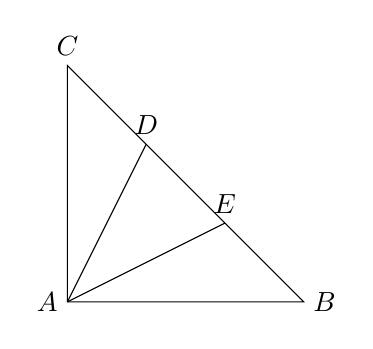
\begin{tikzpicture}
        \coordinate (A) at (0,0);
        \coordinate (B) at (3,0);
        \coordinate (C) at (0,3);
        \coordinate (D) at (1,2);
        \coordinate (E) at (2,1);

        \draw (A) -- (B) -- (C) -- cycle;
        \draw (A) -- (D);
        \draw (A) -- (E);

        \node[left] at (A) {$A$};
        \node[right] at (B) {$B$};
        \node[above] at (C) {$C$};
        \node[above] at (D) {$D$};
        \node[above] at (E) {$E$};
    \end{tikzpicture}
\end{center}
\end{example*}
\begin{solution} \\\\
    First, using the properties of congruent triangles, draw the dotted lines.
    \begin{center}
    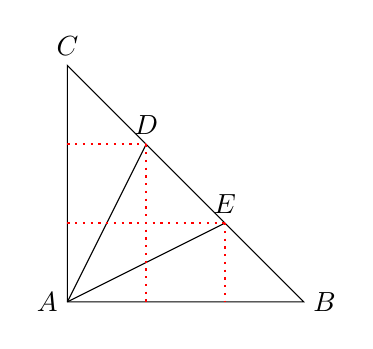
\begin{tikzpicture}
        \coordinate (A) at (0,0);
        \coordinate (B) at (3,0);
        \coordinate (C) at (0,3);
        \coordinate (D) at (1,2);
        \coordinate (E) at (2,1);

        \draw (A) -- (B) -- (C) -- cycle;
        \draw (A) -- (D);
        \draw (A) -- (E);

        \draw[dotted, color=red, thick] (0,2) -- (1,2);
        \draw[dotted, color=red, thick] (0,1) -- (2,1);
        \draw[dotted, color=red, thick] (2,1) -- (2,0);
        \draw[dotted, color=red, thick] (1,2) -- (1,0);

        \node[left] at (A) {$A$};
        \node[right] at (B) {$B$};
        \node[above] at (C) {$C$};
        \node[above] at (D) {$D$};
        \node[above] at (E) {$E$};
    \end{tikzpicture}
    \end{center}
    Let $AB = 3a$ and $AC = 3b$. Using Pythagorean Theorem, it is evident that $4a^2 + b^2 = 1 - 2\sin\theta\cos\theta$ and $a^2 + 4b^2 = 1 + 2\sin\theta\cos\theta$. In other words, $a^2 + b^2 = \frac{2}{5}$.
    \[
    \therefore BC = 9 \cdot \frac{2}{5} = \boxed{\frac{18}{5}}
    \]
\end{solution}

\newpage
\begin{example*}
    If the point $\left( a + \cos\theta, \frac{a}{2} + \sin\theta \right)$ is in the circle $x^2 + y^2 = 4$, find the range of value $a$.
\end{example*}
\begin{solution} \\\\
    Let the point $\left( a + \cos\theta, \frac{a}{2} + \sin\theta \right)$ be $(x,y)$.
    \begin{align*}
        x - a &= \cos\theta \\
        y - \frac{a}{2} &= \sin\theta
        \\\\
        \therefore (x - a)^2 + \left( y - \frac{a}{2} \right)^2 &= 1
    \end{align*}
    The situation could be graphed.
    \begin{center}
        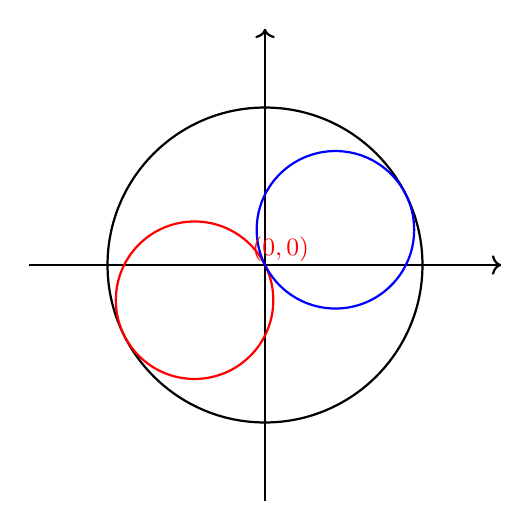
\begin{tikzpicture}
            \draw[thick,->] (-3,0) -- (3,0);
            \draw[thick,->] (0,-3) -- (0,3);
            
            \draw[thick] (0,0) circle (2);
            \draw[red, thick] (-0.8944,-0.4472) circle (1);
            \draw[blue, thick] (0.8944,0.4472) circle (1);
            
            \node[red] at (0.2,0.2) {\small$(0,0)$};
        \end{tikzpicture}
    \end{center}
    Using the distance formula,
    \begin{align*}
        0 \le \sqrt{a^2 + \left( \frac{a}{2} \right)^2} &\le 1 \\
        0 \le a^2 + \left( \frac{a}{2} \right)^2 &\le 1 \\
        0 \le \frac{5a^2}{4} &\le 1 \\
        0 \le a^2 &\le \frac{4}{5} \\
        \boxed{-\frac{2\sqrt{5}}{5} \le a \le \frac{2\sqrt{5}}{5}}&.
    \end{align*}
\end{solution}

\end{document}